\newpage
\lecture{3}{Продолжение борелевской истории и теорема Дынкина.}

\subsection{Структура минимальной сигма-алгебры.}

\begin{exercise}
    Пусть $\F$~--- семейство всех конечных подмножеств множества $X$. Найти $\sigma(\F)$.
\end{exercise}

\begin{solution}
    По определению $\sigma$"=алгебры $\forall A_1,\,A_2,\,\ldots\in\sigma(\F):\ \bigcup\limits_
        {n=1}^{\infty}A_n\in\sigma(\F)$. В частности, это верно для $\forall A_1, \, A_2,\,\ldots\in\F\Rightarrow$ в $\sigma(\F)$
    войдут все не более чем счётные подмножества множества $X$. Кроме того, $\forall A\in\sigma(\F)$ выполнено, что $A^C=X\setminus A\in\sigma(\F)
        \Rightarrow$ в $\sigma(\F)$ войдут также дополнения всех не более чем счётных множеств.

    Итак, $\CG=\{A\subset X:\ A \text{ или } A^C\text{ не более чем счётно}\}\subset\sigma(\F)$.
    Проверим что $\CG$~--- $\sigma$"=алгебра.
    \begin{enumerate}[label=\arabic*\degree.]
        \item $\varnothing\in\CG$~--- очевидно.
        \item $\forall A\in\CG:\ A^C\in\CG$ по построению.
        \item Если доказать, что $\forall A,\, B\in\CG:\ A\cap B\in\CG$, то сразу следует, что и
              $A\cup B = (A\cup B)^{CC}=(A^C\cap B^C)^C\in\CG$ (и наоборот, можно доказать лишь замкнутость по объединению и
              из неё сразу следует замкнутость по пересечению).

              Докажем сразу, что $\forall A_1,\,\ldots,\, A_n,\, \ldots\in\CG$ выполнено $\bigcup\limits_{n=1}^{\infty}A_n\in\CG$,
              то есть докажем разом замкнутость и то, что это именно $\sigma$"=алгебра.
              \begin{enumerate}[label=(a)]
                  \item Пусть $\forall n\in\N\ A_n$ не более чем счётно, тогда $\bigcup\limits_{n=1}^{\infty}A_n\in\CG$ так как
                        объединение так же не более чем счётно.
                  \item Если (a) не выполнено, то $\exists n\in\N:\ A_n$~--- более чем счётно, но так как $A_n\in\CG$, то
                        $A_n^C$~--- не более чем счётно, тогда
                        \[
                            \bigcup_{k=1}^{\infty}A_k=\left(\bigcup_{k=1}^{\infty}A_k\right)^{CC}=
                            \left(\bigcap_{k=1}^{\infty}A_k^C\right)^C.
                        \]
                        Теперь заметим, что в силу свойств пересечения $\bigcap\limits_{k=1}^{\infty}A_k^C\subset A_n^C$, то есть
                        $\bigcap\limits_{k=1}^{\infty}A_k^C$ тоже не более чем счётно, а значит $\bigcup\limits_{k=1}^{\infty}A_k\in\CG$,
                        так как его дополнение не более чем счётно.
              \end{enumerate}
    \end{enumerate}

    Тогда из $\F\subset \CG$ следует, что $\sigma(\F)\subset\CG$
    в силу минимальности по вложению $\sigma(\F)$. Откуда следует, что $\sigma(\F)=\CG$.

\end{solution}

\subsection{Структура борелевской сигма-алгебры.}

Напомним кратко понятия. $K_d$~--- семейство всех клеток в $\R^d$.
Борелевская сигма-алгебра $\FB(\R^d)=\sigma(\tau)$, где $\tau$~--- семейство всех открытых
множеств $U\subset  \R^d$, то есть, так называемая <<евклидова топология>>.

\begin{definition}
    Множество называется \mdef{борелевским} тогда и только тогда, когда оно является элементом
    борелевской сигма-алгебры.
\end{definition}

\begin{claim}
    $\sigma(K_d)=\FB(\R^d)$

    \begin{proof}

        Заметим, что $K_d\subset \FB(\R^d)$, в самом деле
        \[
            K = I_1\times\ldots\times I_d=
            =(I_1\times\R\times\ldots\times\R)\cap
            (\R\times I_2\times\ldots\times \R)\cap\ldots\cap
            (\R\times\R\times\ldots\times I_d),
        \]
        то есть представляем клетку как пересечение <<полос>> (см. рисунок \ref{fig:tapes}).

        \begin{figure}[!ht]
            \centering
            

\tikzset{every picture/.style={line width=0.75pt}} %set default line width to 0.75pt        

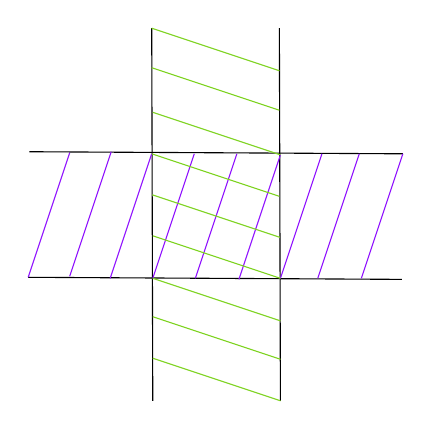
\begin{tikzpicture}[x=0.75pt,y=0.75pt,yscale=-1,xscale=1]
%uncomment if require: \path (0,300); %set diagram left start at 0, and has height of 300

%Straight Lines [id:da17779875153300684] 
\draw    (199.5,50.25) -- (200,229.75) ;
%Straight Lines [id:da5767108711840261] 
\draw    (261,50.25) -- (261.5,229.75) ;
%Straight Lines [id:da8359252951087524] 
\draw    (320.5,110.75) -- (140.5,109.75) ;
%Straight Lines [id:da012133851669587026] 
\draw    (320,171.25) -- (140,170.25) ;
%Straight Lines [id:da6518929305176595] 
\draw [color={rgb, 255:red, 144; green, 19; blue, 254 }  ,draw opacity=1 ]   (140,170.25) -- (160,110.25) ;
%Straight Lines [id:da6820013174751431] 
\draw [color={rgb, 255:red, 144; green, 19; blue, 254 }  ,draw opacity=1 ]   (160,169.75) -- (180,109.75) ;
%Straight Lines [id:da9627497949504988] 
\draw [color={rgb, 255:red, 144; green, 19; blue, 254 }  ,draw opacity=1 ]   (179.5,170.75) -- (199.5,110.75) ;
%Straight Lines [id:da5944146628446789] 
\draw [color={rgb, 255:red, 144; green, 19; blue, 254 }  ,draw opacity=1 ]   (200,170.75) -- (220,110.75) ;
%Straight Lines [id:da5398838559502555] 
\draw [color={rgb, 255:red, 144; green, 19; blue, 254 }  ,draw opacity=1 ]   (220.5,170.75) -- (240.5,110.75) ;
%Straight Lines [id:da06972864594522532] 
\draw [color={rgb, 255:red, 144; green, 19; blue, 254 }  ,draw opacity=1 ]   (241.5,171.25) -- (261.5,111.25) ;
%Straight Lines [id:da7136092221341968] 
\draw [color={rgb, 255:red, 144; green, 19; blue, 254 }  ,draw opacity=1 ]   (261.5,170.75) -- (281.5,110.75) ;
%Straight Lines [id:da24228637647643714] 
\draw [color={rgb, 255:red, 144; green, 19; blue, 254 }  ,draw opacity=1 ]   (279.5,170.75) -- (299.5,110.75) ;
%Straight Lines [id:da9663546970087853] 
\draw [color={rgb, 255:red, 144; green, 19; blue, 254 }  ,draw opacity=1 ]   (300.5,170.75) -- (320.5,110.75) ;
%Straight Lines [id:da5148075032323687] 
\draw [color={rgb, 255:red, 126; green, 211; blue, 33 }  ,draw opacity=1 ]   (199.5,50.25) -- (261,70.75) ;
%Straight Lines [id:da42145939898062923] 
\draw [color={rgb, 255:red, 126; green, 211; blue, 33 }  ,draw opacity=1 ]   (199.5,69.25) -- (261,89.75) ;
%Straight Lines [id:da5408897879376247] 
\draw [color={rgb, 255:red, 126; green, 211; blue, 33 }  ,draw opacity=1 ]   (200,90.75) -- (261.5,111.25) ;
%Straight Lines [id:da040421339799014744] 
\draw [color={rgb, 255:red, 126; green, 211; blue, 33 }  ,draw opacity=1 ]   (199.5,110.75) -- (261,131.25) ;
%Straight Lines [id:da08939729925939699] 
\draw [color={rgb, 255:red, 126; green, 211; blue, 33 }  ,draw opacity=1 ]   (199.75,130.5) -- (261.25,151) ;
%Straight Lines [id:da9111929519111481] 
\draw [color={rgb, 255:red, 126; green, 211; blue, 33 }  ,draw opacity=1 ]   (200,150.25) -- (261.5,170.75) ;
%Straight Lines [id:da33836168419183643] 
\draw [color={rgb, 255:red, 126; green, 211; blue, 33 }  ,draw opacity=1 ]   (200,170.75) -- (261.5,191.25) ;
%Straight Lines [id:da521634480582023] 
\draw [color={rgb, 255:red, 126; green, 211; blue, 33 }  ,draw opacity=1 ]   (200,189.25) -- (261.5,209.75) ;
%Straight Lines [id:da9952121237853362] 
\draw [color={rgb, 255:red, 126; green, 211; blue, 33 }  ,draw opacity=1 ]   (200,209.25) -- (261.5,229.75) ;




\end{tikzpicture}

            \caption{Двумерные полоски.}
            \label{fig:tapes}
        \end{figure}

        Теперь посмотрим на промежутки:

        \begin{align*}
            I_1=\left[
            \begin{array}{ll}
                (a,\, b) \text{~--- открытое} \Rightarrow\in\FB(\R),\\
                \left[ a,\, b\right)=\bigcap\limits_{n=1}^{\infty} 
                \left(a-\dfrac{1}{n},\, b\right)\Rightarrow \in\FB(\R),\\ 
                \left( a,\, b\right]\text{~--- аналогично}\in\FB(\R),\\
                \left[a,\, b\right]\text{~--- дополнение к открытому}\Rightarrow\in\FB(\R).
            \end{array}
            \right .
        \end{align*}

        Аналогично множества $(I_1\times\R\times\ldots\times\R),\,
        (\R\times I_2\times\ldots\times \R),\,\ldots,\,
        (\R\times\R\times\ldots\times I_d)\in\FB(\R^d)$. А следовательно и их пересечение является
        борелевским множеством. 

        Итак, доказано, что $K_d\subset \FB(\R^d)\Rightarrow \sigma(K_d)\subset\FB(\R^d)$.

        Докажем теперь, что $\FB(\R^d)\subset \sigma(K_d)$. Так как 
        $\FB(\R^d)=\sigma(\tau)$ (см. определение), то достаточно доказать, что 
        $\tau\subset \sigma(K_d)$, в самом деле, если $\tau\subset \sigma(K_d)$, то 
        $\sigma(\tau)\subset \sigma(K_d)$ в силу минимальности $\sigma(\tau)$ по вложению.

        Пусть $U\in\tau$. Докажем, что $U\in\sigma(K_d)$.

        \begin{figure}[!ht]
            \centering
            

\tikzset{every picture/.style={line width=0.75pt}} %set default line width to 0.75pt        

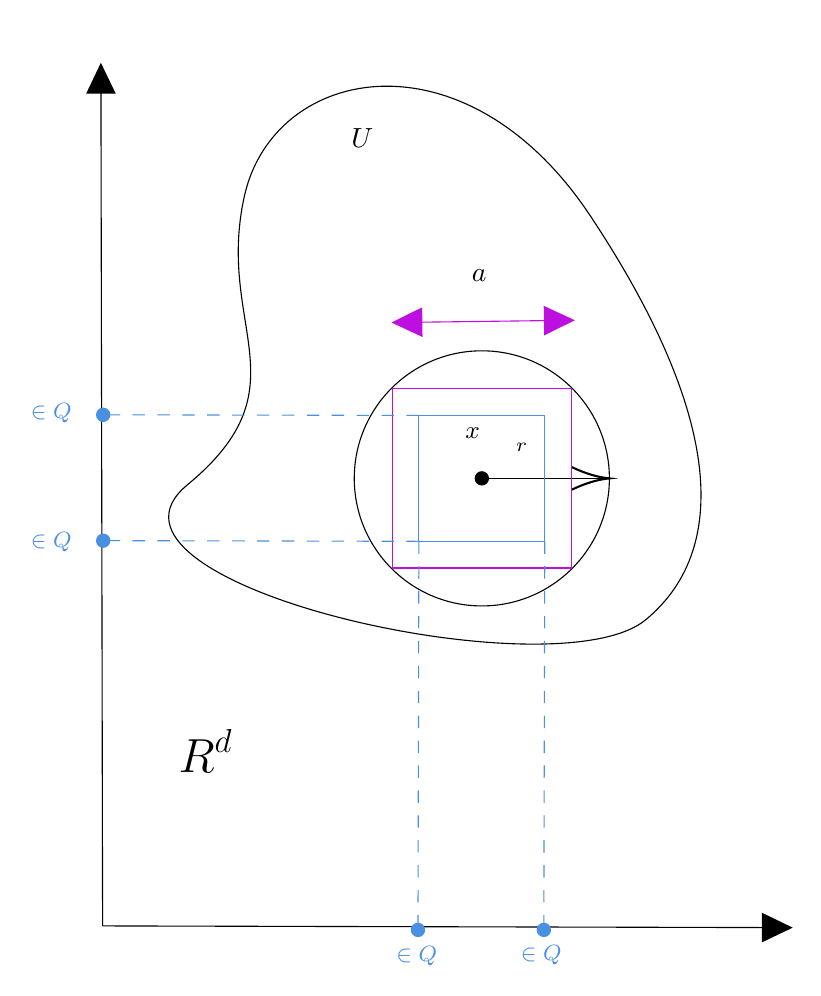
\begin{tikzpicture}[x=1.25pt,y=1.25pt,yscale=-1,xscale=1]
%uncomment if require: \path (0,300); %set diagram left start at 0, and has height of 300

%Straight Lines [id:da3891295536787627] 
\draw    (40.01,23.75) -- (40.5,270.25) ;
\draw [shift={(40,20.75)}, rotate = 89.89] [fill={rgb, 255:red, 0; green, 0; blue, 0 }  ][line width=0.08]  [draw opacity=0] (8.93,-4.29) -- (0,0) -- (8.93,4.29) -- cycle    ;
%Straight Lines [id:da8753009787612205] 
\draw    (40.5,270.25) -- (237,270.74) ;
\draw [shift={(240,270.75)}, rotate = 180.14] [fill={rgb, 255:red, 0; green, 0; blue, 0 }  ][line width=0.08]  [draw opacity=0] (8.93,-4.29) -- (0,0) -- (8.93,4.29) -- cycle    ;
%Shape: Polygon Curved [id:ds2642387232563135] 
\draw   (81.5,59.25) .. controls (90,21.25) and (145.5,10.75) .. (181.5,65) .. controls (217.5,119.25) and (223.5,160.25) .. (197.5,181.75) .. controls (171.5,203.25) and (30.5,171.25) .. (65,142.75) .. controls (99.5,114.25) and (73,97.25) .. (81.5,59.25) -- cycle ;
%Shape: Circle [id:dp4238801266140033] 
\draw   (113.25,140.88) .. controls (113.25,120.51) and (129.76,104) .. (150.13,104) .. controls (170.49,104) and (187,120.51) .. (187,140.88) .. controls (187,161.24) and (170.49,177.75) .. (150.13,177.75) .. controls (129.76,177.75) and (113.25,161.24) .. (113.25,140.88) -- cycle ;
%Flowchart: Connector [id:dp3582654588008982] 
\draw  [color={rgb, 255:red, 0; green, 0; blue, 0 }  ,draw opacity=1 ][fill={rgb, 255:red, 0; green, 0; blue, 0 }  ,fill opacity=1 ] (148.22,140.88) .. controls (148.22,139.82) and (149.07,138.97) .. (150.13,138.97) .. controls (151.18,138.97) and (152.03,139.82) .. (152.03,140.88) .. controls (152.03,141.93) and (151.18,142.78) .. (150.13,142.78) .. controls (149.07,142.78) and (148.22,141.93) .. (148.22,140.88) -- cycle ;
%Straight Lines [id:da9832211334903285] 
\draw    (150.13,140.88) -- (185,140.88) ;
\draw [shift={(187,140.88)}, rotate = 180] [color={rgb, 255:red, 0; green, 0; blue, 0 }  ][line width=0.75]    (10.93,-3.29) .. controls (6.95,-1.4) and (3.31,-0.3) .. (0,0) .. controls (3.31,0.3) and (6.95,1.4) .. (10.93,3.29)   ;
%Shape: Square [id:dp1714725879106831] 
\draw  [color={rgb, 255:red, 189; green, 16; blue, 224 }  ,draw opacity=1 ] (124.23,114.98) -- (176.02,114.98) -- (176.02,166.77) -- (124.23,166.77) -- cycle ;
%Shape: Square [id:dp79912912986395] 
\draw  [color={rgb, 255:red, 74; green, 144; blue, 226 }  ,draw opacity=1 ] (131.93,122.68) -- (168.32,122.68) -- (168.32,159.07) -- (131.93,159.07) -- cycle ;
%Straight Lines [id:da4855369317833904] 
\draw [color={rgb, 255:red, 74; green, 144; blue, 226 }  ,draw opacity=1 ] [dash pattern={on 4.5pt off 4.5pt}]  (131.93,159.07) -- (131.67,269.5) ;
%Straight Lines [id:da5174923462359278] 
\draw [color={rgb, 255:red, 74; green, 144; blue, 226 }  ,draw opacity=1 ] [dash pattern={on 4.5pt off 4.5pt}]  (168.32,159.07) -- (168.05,269.5) ;
%Straight Lines [id:da6360615454864518] 
\draw [color={rgb, 255:red, 74; green, 144; blue, 226 }  ,draw opacity=1 ] [dash pattern={on 4.5pt off 4.5pt}]  (131.93,122.68) -- (40.67,122.5) ;
%Straight Lines [id:da9001259383630189] 
\draw [color={rgb, 255:red, 74; green, 144; blue, 226 }  ,draw opacity=1 ] [dash pattern={on 4.5pt off 4.5pt}]  (131.93,159.07) -- (40.67,158.88) ;
%Flowchart: Connector [id:dp12595981061799733] 
\draw  [color={rgb, 255:red, 74; green, 144; blue, 226 }  ,draw opacity=1 ][fill={rgb, 255:red, 74; green, 144; blue, 226 }  ,fill opacity=1 ] (129.76,271.41) .. controls (129.76,270.35) and (130.61,269.5) .. (131.67,269.5) .. controls (132.72,269.5) and (133.57,270.35) .. (133.57,271.41) .. controls (133.57,272.46) and (132.72,273.31) .. (131.67,273.31) .. controls (130.61,273.31) and (129.76,272.46) .. (129.76,271.41) -- cycle ;
%Flowchart: Connector [id:dp1465179006625632] 
\draw  [color={rgb, 255:red, 74; green, 144; blue, 226 }  ,draw opacity=1 ][fill={rgb, 255:red, 74; green, 144; blue, 226 }  ,fill opacity=1 ] (166.14,271.41) .. controls (166.14,270.35) and (167,269.5) .. (168.05,269.5) .. controls (169.1,269.5) and (169.96,270.35) .. (169.96,271.41) .. controls (169.96,272.46) and (169.1,273.31) .. (168.05,273.31) .. controls (167,273.31) and (166.14,272.46) .. (166.14,271.41) -- cycle ;
%Flowchart: Connector [id:dp431077373880995] 
\draw  [color={rgb, 255:red, 74; green, 144; blue, 226 }  ,draw opacity=1 ][fill={rgb, 255:red, 74; green, 144; blue, 226 }  ,fill opacity=1 ] (38.76,158.88) .. controls (38.76,157.83) and (39.61,156.98) .. (40.67,156.98) .. controls (41.72,156.98) and (42.57,157.83) .. (42.57,158.88) .. controls (42.57,159.94) and (41.72,160.79) .. (40.67,160.79) .. controls (39.61,160.79) and (38.76,159.94) .. (38.76,158.88) -- cycle ;
%Flowchart: Connector [id:dp4846052501292355] 
\draw  [color={rgb, 255:red, 74; green, 144; blue, 226 }  ,draw opacity=1 ][fill={rgb, 255:red, 74; green, 144; blue, 226 }  ,fill opacity=1 ] (38.76,122.5) .. controls (38.76,121.45) and (39.61,120.59) .. (40.67,120.59) .. controls (41.72,120.59) and (42.57,121.45) .. (42.57,122.5) .. controls (42.57,123.55) and (41.72,124.41) .. (40.67,124.41) .. controls (39.61,124.41) and (38.76,123.55) .. (38.76,122.5) -- cycle ;
%Straight Lines [id:da3568745740929704] 
\draw [color={rgb, 255:red, 189; green, 16; blue, 224 }  ,draw opacity=1 ]   (127,95.8) -- (174,95.2) ;
\draw [shift={(177,95.17)}, rotate = 539.28] [fill={rgb, 255:red, 189; green, 16; blue, 224 }  ,fill opacity=1 ][line width=0.08]  [draw opacity=0] (8.93,-4.29) -- (0,0) -- (8.93,4.29) -- cycle    ;
\draw [shift={(124,95.83)}, rotate = 359.28] [fill={rgb, 255:red, 189; green, 16; blue, 224 }  ,fill opacity=1 ][line width=0.08]  [draw opacity=0] (8.93,-4.29) -- (0,0) -- (8.93,4.29) -- cycle    ;

% Text Node
\draw (111.64,38.86) node [anchor=north west][inner sep=0.75pt]   [align=left] {$\displaystyle U$};
% Text Node
\draw (159.29,129.93) node [anchor=north west][inner sep=0.75pt]  [font=\scriptsize] [align=left] {$\displaystyle r$};
% Text Node
\draw (124.67,275.33) node [anchor=north west][inner sep=0.75pt]  [font=\footnotesize,color={rgb, 255:red, 74; green, 144; blue, 226 }  ,opacity=1 ] [align=left] {$\displaystyle \in \mathbb{Q}$};
% Text Node
\draw (160.67,275) node [anchor=north west][inner sep=0.75pt]  [font=\footnotesize,color={rgb, 255:red, 74; green, 144; blue, 226 }  ,opacity=1 ] [align=left] {$\displaystyle \in \mathbb{Q}$};
% Text Node
\draw (19,118.33) node [anchor=north west][inner sep=0.75pt]  [font=\footnotesize,color={rgb, 255:red, 74; green, 144; blue, 226 }  ,opacity=1 ] [align=left] {$\displaystyle \in \mathbb{Q}$};
% Text Node
\draw (19,155.67) node [anchor=north west][inner sep=0.75pt]  [font=\footnotesize,color={rgb, 255:red, 74; green, 144; blue, 226 }  ,opacity=1 ] [align=left] {$\displaystyle \in \mathbb{Q}$};
% Text Node
\draw (144.62,125.57) node [anchor=north west][inner sep=0.75pt]  [font=\small] [align=left] {$\displaystyle x$};
% Text Node
\draw (146.48,79.86) node [anchor=north west][inner sep=0.75pt]   [align=left] {$\displaystyle a$};
% Text Node
\draw (61.71,212.71) node [anchor=north west][inner sep=0.75pt]  [font=\LARGE] [align=left] {$\displaystyle \mathbb{R}^{d}$};


\end{tikzpicture}

            \caption{Множество $U$.}
            \label{fig:upic}
        \end{figure}

        $U$ открытое, поэтому $\forall x\in U\ \exists r>0:\ B_r(x)\subset U$, где $B_r(x)$~--- 
        $d$"=мерный шар радиуса $r$ с центром в точке $x$. Поймем какого размера должен быть 
        $d$"=мерный куб, чтобы его можно было вписать в данный шар. Должно выполнится следующее 
        неравенство: $\left(\dfrac{a}{2}\right)^2\cdot d\leqslant r^2$, где $a$~--- искомая сторона
        куба (неравенство следует из теоремы Пифагора: полудиагональ куба складывается из $d$ частей, 
        каждая длиной $\frac{a}{2}$). Откуда $a\leqslant \dfrac{2r}{\sqrt{d}}$. Таким образов любое 
        открытое множество можно представить в виде объединения таких кубиков (на рисунке \ref{fig:upic} это розовый квадрат),
        а кубики уже принадлежат семейству клеточных множеств.
        
        Но возникает проблема: такое объединение кубиков может оказаться более чем счётным, поэтому сделаем финт ушами:
        сожмём кубик так, чтобы координаты его граней были рациональными (на рисунке это синий квадратик) и обзовем его $Q_x$.
        Множество таких кубов счётно, так как все такие кубы можно параметризовать точками $\Q^{2d}\Rightarrow$ данное семейство 
        счётно. 

        Тогда $\forall x\in U$ поставим в соответствие соответствующий куб $Q_x\subset B_r(x)\subset U$ и 
        $U=\bigcup\limits_{x\in U}\{x\}\subset \bigcup\limits_{x\in U}Q_x$~--- представимо в виде 
        не более чем счётного объединения, так как число кубов счётно и значит $U=\bigcup\limits_{x\in U}Q_x\in\sigma(K_d)$.

    \end{proof} 
\end{claim}

\subsection{Теорема Дынкина.}

\begin{definition}
    Семейство $\F\subset \CP(X)$ называется:
    \begin{enumerate}[label=\arabic*)]
        \item \mdef{$\pi$"=системой}, если $\forall A,\, B\in\F$ выполнено, что $A\cap B\in\F$;
        \item \mdef{$\lambda$"=системой}, если, во-первых, $\varnothing\in\F$, во-вторых,
        $\forall A\in\F$ выполнено, что $A^C\in\F$, а также для любых попарно непересекающихся 
        $D_1,\, \ldots,\, D_n,\,\ldots\in\F$ выполнено $\bigsqcup\limits_{k=1}^{\infty} D_k\in\F$.
    \end{enumerate}
\end{definition}

\begin{exercise}
    $\lambda$"=система в общем случае не всегда является $\pi$"=системой. Например, пусть 
    $X=\{1,\,2,\,3,\,4\}$ и 
    \[
        \F = \{\varnothing,\, X,\, \{1,\,2\},\, \{1,\,3\},\,\{1,\,4\},\,\{2,\,3\},\,\{2,\,4\},\,\{3,\,4\}\}.    
    \]
    Легко видеть, что это $\lambda$"=система, но не $\pi$"=система, так как $\F$ не замкнута относительно пересечения.
\end{exercise}

\begin{exercise}
    Другой пример. Пусть $X=\R^2,\ \F = \{\R\times A:\ A\subset \R\}\cup \{A\times \R:\ A\subset \R\}$~---
    семейство горизонтальных и вертикальных полос.
    \begin{enumerate}
        \item $\F$~--- не $\pi$"=система, так как $(\R\times A)\cap (B\times \R)=B\times A\notin \F,\ A,\, B\neq \R$.
        \item Легко видеть, что $\F$~--- $\lambda$"=система.
    \end{enumerate}
\end{exercise}

На прошлой лекции было доказано следующее утверждение (теперь в новой терминологии):
\begin{claim}
    $\F\subset\CP(X)$ является $\sigma$"=алгеброй тогда и только тогда, когда $\F$ 
    одновременно является $\pi$"=системой и $\lambda$"=системой.
\end{claim}

\begin{figure}[!ht]
    \centering
    \tikzset{every picture/.style={line width=0.75pt}} %set default line width to 0.75pt        

\begin{tikzpicture}[x=0.75pt,y=0.75pt,yscale=-1,xscale=1]
%uncomment if require: \path (0,300); %set diagram left start at 0, and has height of 300

%Shape: Ellipse [id:dp25713279954981605] 
\draw[pattern=north east lines, pattern color=LimeGreen]   (46,113.25) .. controls (46,69.48) and (105.77,34) .. (179.5,34) .. controls (253.23,34) and (313,69.48) .. (313,113.25) .. controls (313,157.02) and (253.23,192.5) .. (179.5,192.5) .. controls (105.77,192.5) and (46,157.02) .. (46,113.25) -- cycle ;
%Shape: Circle [id:dp054806241779318254] 
\draw[fill=white]   (150.2,98.7) .. controls (150.2,78.21) and (166.81,61.6) .. (187.3,61.6) .. controls (207.79,61.6) and (224.4,78.21) .. (224.4,98.7) .. controls (224.4,119.19) and (207.79,135.8) .. (187.3,135.8) .. controls (166.81,135.8) and (150.2,119.19) .. (150.2,98.7) -- cycle ;
%Shape: Circle [id:dp27458954298091864] 
\draw[pattern=north east lines, pattern color=LimeGreen]    (108.6,119.5) .. controls (108.6,99.01) and (125.21,82.4) .. (145.7,82.4) .. controls (166.19,82.4) and (182.8,99.01) .. (182.8,119.5) .. controls (182.8,139.99) and (166.19,156.6) .. (145.7,156.6) .. controls (125.21,156.6) and (108.6,139.99) .. (108.6,119.5) -- cycle ;
%Shape: Path Data [id:dp6741602689881148] 
\draw[pattern=north west lines, pattern color=RubineRed]   (182.8,119.1) .. controls (182.8,124.62) and (181.59,129.86) .. (179.43,134.56) .. controls (162.72,130.96) and (150.2,116.09) .. (150.2,98.3) .. controls (150.2,92.78) and (151.41,87.54) .. (153.57,82.84) .. controls (170.28,86.44) and (182.8,101.31) .. (182.8,119.1) -- cycle ;

% Text Node
\draw (124,130.2) node [anchor=north west][inner sep=0.75pt]   [align=left] {$\displaystyle A$};
% Text Node
\draw (202.4,100.6) node [anchor=north west][inner sep=0.75pt]   [align=left] {$\displaystyle N$};


\end{tikzpicture}


    \caption{К теореме Дынкина (\ref{theorem:dynkin})}
    \label{fig:sets}
\end{figure}

\begin{theorem}[Дынкин]
    \label{theorem:dynkin}

    Пусть $\F\subset\CP(X)$~--- $\pi$"=система, $\CE\subset\CP(X)$~--- $\lambda$"=система и
    $\F\subset\CE$. Тогда $\sigma(\F)\subset\CE$ (равенство возможно).

    \begin{proof}
        Пусть $\CD\subset \CP(X)$~--- пересечение всех $\lambda$"=систем $\CG\subset\CP(X)$, 
        таких что $\F\subset\CG$. Докажем, что $\sigma(\F)\subset\CD$, для этого достаточно доказать, 
        что $\CD$ является $\sigma$"=алгеброй (снова в силу минимальности).

        Заметим, что $\CD$~--- $\lambda$"=система (доказывается так же как и факт о том, что пересечение сигма-алгебр является
        сигма-алгеброй). Тогда достаточно показать, что $\CD$~--- $\pi$"=система, то есть, что 
        $\forall M,\, N\in\CD$ выполняется, что $M\cap N\in\CD$.

        Введем обозначение: $\CH(M)=\{N\in\CD:\: M\cap N\in\CD\}$, где $M$~--- любой элемент $\CD$. То есть 
        условие о замкнутости по пересечению можно переформулировать так: $\forall M\in\CD$ выполнено $\CH(M)=\CD$.

        \begin{lemma}
            $\forall N\in\CD$ верно, что $\CH(N)$ является $\lambda$"=системой.

            \begin{proof}
                Во-первых, $\varnothing\in\CH(N)$, так как $\forall M\in\CD:\ \varnothing\cap M=\varnothing\in\CD$ по определению.

                Во-вторых, докажем, что $\CH(N)$ замкнуто относительно взятия дополнений. Пусть $A\in\CH(N)$. 
                Заметим, что
                \begin{equation}
                    \label{eq:lemmastate}
                    A\in\CH(N)\ \Leftrightarrow\ A\cap N\in\CD.
                \end{equation}
                И в частности 
                \[
                    A^C\in\CH(N)\ \Leftrightarrow\ A^C\cap N\in\CD.    
                \]
                Правое условие, в силу того, что $\CD$~--- $\lambda$"=система эквивалентно тому, что 
                $(A^C\cap N)^C\in\CD$ (из замкнутости по дополнению). Но $(A^C\cap N)^C=A\cup N^C=(A\cap N)\sqcup N^C\in\CD$ 
                (см. рис. \ref{fig:sets}). Итак, $A^C\in\CH(N)$.

                Докажем замкнутость относительно дизъюнктных объединений. Пусть 
                $A_1,\,\ldots,\,A_n,\,\ldots\in\CH(N)$ попарно не пересекаются. Тогда:
                \[
                    \left(\bigsqcup_{n=1}^{\infty}A_n\right)\cap N=\bigsqcup_{n=1}^{\infty}\left(A_n\cap N\right)\in \CD,
                \]
                так как $A_n\cap N\in\CD$ (см. условие \eqref{eq:lemmastate}) и $\CD$~--- $\lambda$"=система.

            \end{proof}
        \end{lemma}

        Пусть $M\in\F\subset\CD$ (по построению). Зададимся вопросом: для каких $N\in\CD$ выполнено, что $M\cap N\in\CD$?
        Если $N\in\F$, то $M\cap N\in\F$, так как $\F$~--- $\pi$"=система. Поэтому $\forall N\in\F$
        выполнено $N\in\CH(M)$, то есть $\F\subset\CH(M)$, а значит $\CH(M)$~--- одна из $\lambda$"=систем, включающих в себя 
        $\F$, следовательно, в силу минимальности по вложению, $\CD\subset\CH(M)$ для $\forall M\in\F$, 
        то есть $\forall N\in\CD,\, \forall M\in\F$ выполнено $M\cap N\in\CD$. А значит $\forall N\in\CD$ выполнено $\F\subset\CH(N)$, и 
        снова в силу минимальности $\CD\subset \CH(N)$. Итак, $\forall N,\, M\in\CD$ выполнено $M\cap N\in\CD$.
        
    \end{proof}
\end{theorem}

